%---------------------------------------------------------
%	PRESENTATION BODY SLIDES
%---------------------------------------------------------
\section{Дуальная структура} % Note all sections and subsections are automatically placed in your table of contents
%------------------------------------------------
\begin{frame}
	\frametitle{Дуальная структура}
	При разработке структуры, удовлетворяющей требованиям, предъявляемым к частицам с различным зарядом, важно создать перестраиваемую структуру без внесения конструктивных изменений. Мы назвали такую структуру -- \textit{дуальной}.
	\vspace{2em} 
	\begin{columns}
		\begin{column}{0.5\textwidth}
			\raggedright
			\adjustbox{valign=t}{\begin{minipage}[t]{\linewidth}
					\centering \textbf{Тяжёлые ионы}\\
					обладают более выраженным эффектом разогрева из-за внутрипучкового рассеяния.\\
			\end{minipage}}
		\end{column}
		\hfill
		\begin{column}{0.5\textwidth}
			\raggedright
			\adjustbox{valign=t}{\begin{minipage}[t]{\linewidth}
					\centering{\textbf{Лёгкие частицы}}\\
					влияние критической энергии на динамику сгустка.\\
			\end{minipage}}
		\end{column}
		\begin{column}{0.01\textwidth}
		\end{column}
	\end{columns}		
\end{frame}
%------------------------------------------------
\begin{frame}
	\frametitle{Тяжелоионная опция}
	Особенность кольца для высоко интенсивного пучка тяжелых ионов, состоит в обеспечении высокого времени жизни. Ввиду высокой зарядности частиц, критически важным является влияние внутрипучкового рассеяния (ВПР)
	\begin{equation}
		\frac{1}{\tau_x}=\frac{\pi^2r_0^2v_cm^3N\left(log\right)}{\gamma\Gamma}\left[\frac{\gamma^2\left(D_x^2+\beta_x^2\phi_x^2\right)}{\epsilon_x\beta_x}\right]\int_{0}^{\infty}\frac{d\lambda\ \lambda^\frac{1}{2}\left[a_x\lambda+b_x\right]}{\left(\lambda^3+a\lambda^2+b\lambda+c\right)^\frac{3}{2}}
	\end{equation}
	Общим походом в этом случае являются минимизация бета-функции и дисперсии, а также их регуляризация, что приводит к увеличению времени ВПР в структуре.
\end{frame}
%------------------------------------------------
\begin{frame}
	\frametitle{Регулярная структура}
	\begin{columns}
		\begin{column}{0.3\textwidth}
			\raggedright
			\adjustbox{valign=t}{\begin{minipage}[t]{\linewidth}
					В регулярной структуре $\gamma_{\text{tr}}\simeq\nu_{x}$. \\
					При одинаковой магнитной жесткости $B\rho$ максимальная энергия для легких частиц выше, чем для тяжелых ионов, из-за их соотношения заряд-масса.
			\end{minipage}}
		\end{column}
		\begin{column}{0.7\textwidth}
			\begin{minipage}{\linewidth}
				\centering
				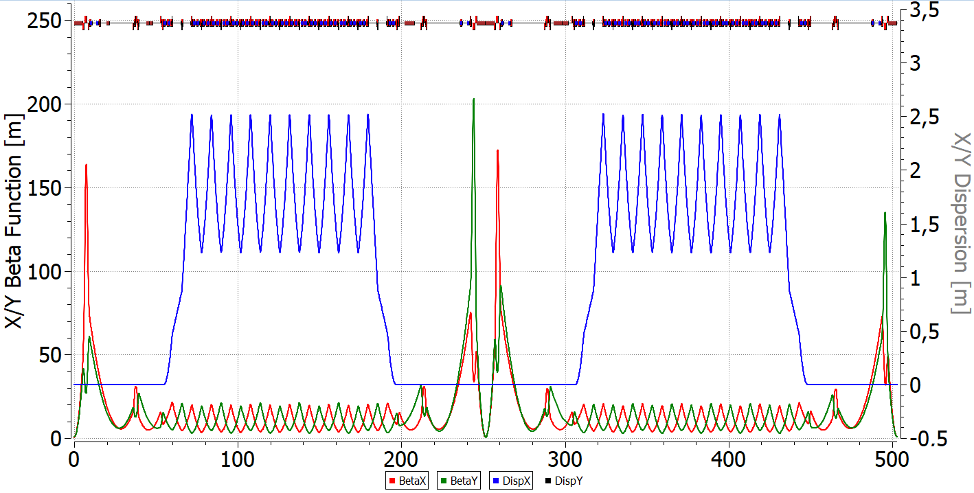
\includegraphics[width=1\linewidth]{images/1_regular}
			\end{minipage}
		\end{column}
	\end{columns}
\end{frame}
%------------------------------------------------
\begin{frame}
\frametitle{Критическая энергия}
Критическая энергия связана с коэффициентом уплотнения орбиты (momentum compaction factor) 
\begin{equation}
	\alpha=\frac{1}{\gamma_{\text{tr}}^2}=\frac{1}{C}\int_{0}^{C}\frac{D\left(s\right)}{\rho\left(s\right)}ds
\end{equation}
Поднятие критической энергии возможно при вариации дисперсии и кривизны.
\newline
\par  Коэффициент уплотнения орбиты для суперпериода при суперпериодической модуляции градиента квадрупольных линз в первом порядке
\begin{equation}
\alpha_s=\frac{1}{{\nu_x}^2}\left\{1+\frac{1}{4\left(1-S/\nu_x\right)}\left(\frac{\bar{R}}{\nu_x}\right)^4\left.\frac{g_k^2}{\left[1-(1-S/\nu_x)^2\right]^2}\right\}\right.
\end{equation}
\end{frame}
%------------------------------------------------
\begin{frame}
	\frametitle{Резонансная структура}
	\begin{columns}
		\begin{column}{0.3\textwidth}
			\raggedright
			\adjustbox{valign=t}{\begin{minipage}[t]{\linewidth}
					Может быть получена из регулярной структуры путем разделения фокусирующих квадруполей на 2 семейства с различными градиентами.		
			\end{minipage}}
		\end{column}
		\begin{column}{0.7\textwidth}
			\begin{minipage}{\linewidth}
				\centering
				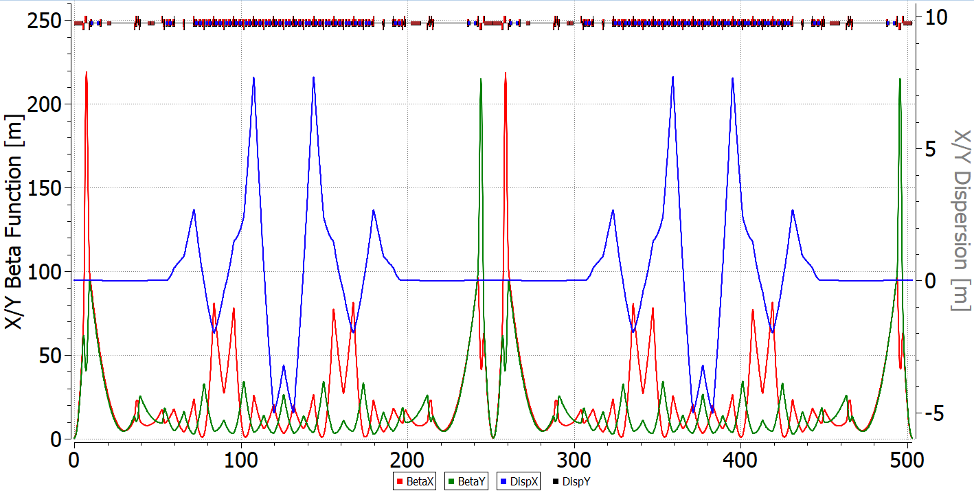
\includegraphics[width=1\linewidth]{images/1_resonant}
			\end{minipage}
		\end{column}
	\end{columns}
\end{frame}
%------------------------------------------------
\begin{frame}
	\frametitle{Комбинированная структура}
	\begin{columns}
		\begin{column}{0.3\textwidth}
			\raggedright
			\adjustbox{valign=t}{\begin{minipage}[t]{\linewidth}
					Реальная арка
					\begin{equation} \label{eq:eta_pk}
						\eta_{\textrm{pk}}=\frac{1}{\gamma_{\textrm{tr}}^2}-\frac{1}{\gamma^2}
					\end{equation}
					\noindent компенсируется аркой с комплексным значением критической энергии
					\begin{equation} \label{eq:eta_kp}
						\eta_{\textrm{kp}}=-\frac{1}{\gamma_{\textrm{tr}}^2}-\frac{1}{\gamma^2}\ \ \ 
					\end{equation}
			\end{minipage}}
		\end{column}
		\begin{column}{0.7\textwidth}
			\begin{minipage}{\linewidth}
				\centering
				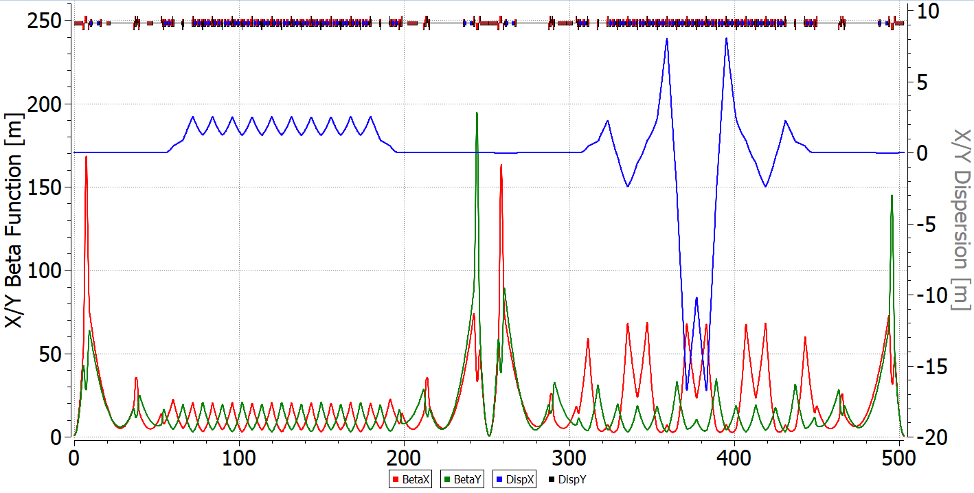
\includegraphics[width=1\linewidth]{images/1_combined}
			\end{minipage}
		\end{column}
	\end{columns}
\end{frame}
%------------------------------------------------
\begin{frame}
	\frametitle{Стохастическое охлаждение и ВПР}
	
	\begin{columns}
		\begin{column}{0.5\textwidth}
			\begin{minipage}{\linewidth}
				\centering
				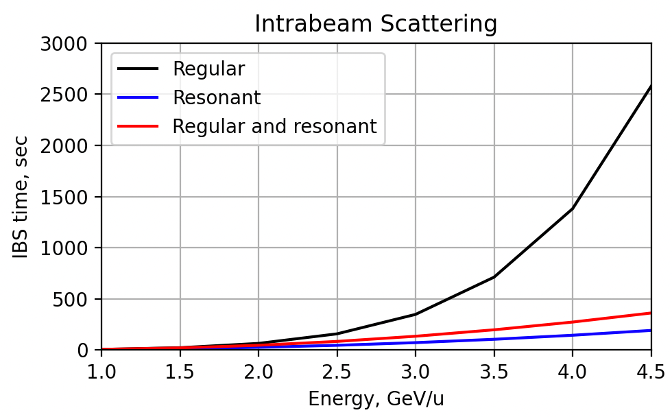
\includegraphics[width=0.8\linewidth]{images/1_IBS}
			\end{minipage}
		\end{column}
		\begin{column}{0.5\textwidth}
			\begin{minipage}{\linewidth}
				\centering
				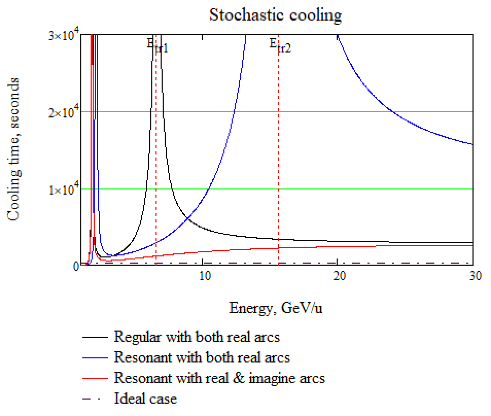
\includegraphics[width=0.8\linewidth]{images/1_SC_wide}
			\end{minipage}
		\end{column}
	\end{columns}
\end{frame}
%------------------------------------------------